\documentclass[tikz,border=6pt]{standalone}
\usepackage{tikz}
\usetikzlibrary{patterns,calc}

\begin{document}
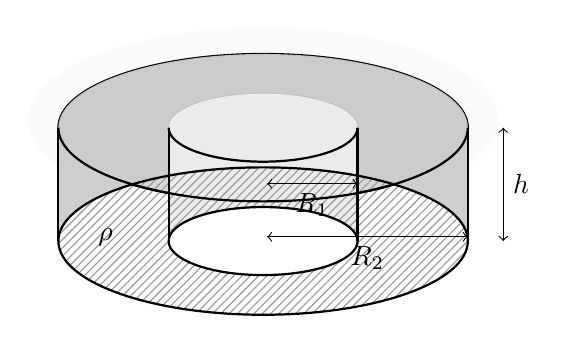
\begin{tikzpicture}[line join=round]

% ===== 参数(按需调整) =====
\def\Rone{1.2}   % 内环外半径 (cm)
\def\Rtwo{2.6}   % 外环内半径 (cm)
\def\h{1.6}      % 高度 h (cm)
\def\yscale{0.36} % 竖直方向压缩比(椭圆的竖半轴 = R*yscale)
\def\proj{0.9}    % 高度投影因子(top ellipse 相对 bottom 的纵向偏移系数)

\pgfmathsetmacro{\topoffset}{\h*\proj} % top ellipse 的中心相对于 bottom 的 y 偏移

% ===== 阴影(底部) =====
\fill[black!8,opacity=0.25] (0,0.1) ellipse ({\Rtwo*1.15} and {\Rtwo*\yscale*1.25});

% ===== 底面椭圆 (bottom) =====
\fill[gray!30] (0,0) ellipse ({\Rtwo} and {\Rtwo*\yscale});
\fill[white]    (0,0) ellipse ({\Rone} and {\Rone*\yscale});
\draw[thick]    (0,0) ellipse ({\Rtwo} and {\Rtwo*\yscale});
\draw[thick]    (0,0) ellipse ({\Rone} and {\Rone*\yscale});

% ===== 外侧壁 (用弧连接 bottom -> top 显示侧面) =====
\path[fill=gray!40,draw=none,opacity=0.95]
  (\Rtwo,0) arc (0:180:{\Rtwo} and {\Rtwo*\yscale})
  -- ++(0,-\topoffset)
  arc (180:0:{\Rtwo} and {\Rtwo*\yscale}) -- cycle;

% ===== 内侧壁 =====
\path[fill=gray!15,draw=none,opacity=0.98]
  (\Rone,0) arc (0:180:{\Rone} and {\Rone*\yscale})
  -- ++(0,-\topoffset)
  arc (180:0:{\Rone} and {\Rone*\yscale}) -- cycle;

% ===== 顶面(top ellipse)并用 pattern 表示导电材料 rho(顶面) =====
\fill[pattern=north east lines,pattern color=black!40] (0,-\topoffset) ellipse ({\Rtwo} and {\Rtwo*\yscale});
\fill[white] (0,-\topoffset) ellipse ({\Rone} and {\Rone*\yscale});

% 顶面轮廓
\draw[thick] (0,-\topoffset) ellipse ({\Rtwo} and {\Rtwo*\yscale});
\draw[thick] (0,-\topoffset) ellipse ({\Rone} and {\Rone*\yscale});

% ===== 前景边缘(下半弧)用于增加立体感 =====
\draw[thick] (\Rtwo,0) arc (0:-180:{\Rtwo} and {\Rtwo*\yscale});
\draw[thick] (\Rone,0)  arc (0:-180:{\Rone} and {\Rone*\yscale});

% ===== 竖直连接线(给出高度感) =====
\draw[thick] ({\Rtwo},0) -- ({\Rtwo},-\topoffset);
\draw[thick] ({-\Rtwo},0) -- ({-\Rtwo},-\topoffset);
\draw[thick] ({\Rone},0) -- ({\Rone},-\topoffset);
\draw[thick] ({-\Rone},0) -- ({-\Rone},-\topoffset);

% ===== 标注 =====
% R2 和 R1(从中心到右侧外轮廓的投影位置)
\draw[<->] (0.05, -\Rtwo*\yscale - 0.45) -- (\Rtwo, -\Rtwo*\yscale - 0.45) node[midway,below] {$R_2$};
\draw[<->] (0.05, -\Rone*\yscale - 0.28) -- (\Rone, -\Rone*\yscale - 0.28) node[midway,below] {$R_1$};

% h 标注
\draw[<->] (\Rtwo+0.45,0) -- (\Rtwo+0.45,-\topoffset) node[midway,right] {$h$};

% rho 标注放在顶面环上
\node at (-2,-\topoffset+0.05) {$\rho$};

% 标题(可选)
% \node[above,font=\bfseries] at (0,0.95) {立体俯视示意图(无需 tikz-3dplot)};

\end{tikzpicture}
\end{document}
